\documentclass[11pt]{article}

\usepackage[margin=1in]{geometry}
\usepackage{amsmath,amssymb}
\usepackage{graphicx}
\usepackage{booktabs}
\usepackage[round]{natbib}
\usepackage[hidelinks]{hyperref}
\usepackage{microtype}
\usepackage{siunitx}
\usepackage{float}
\usepackage{caption}
\usepackage{listings}
\usepackage{xcolor}
\hypersetup{
  pdftitle={ddmtorch: A Differentiable, MPS-Accelerated Toolbox for Drift-Diffusion Model Estimation on Apple Silicon},
  pdfauthor={ChiaAn Lin},
  pdfsubject={Technical report},
  pdfkeywords={drift-diffusion model, Wiener first-passage time, maximum likelihood, hierarchical Bayesian, PyTorch, Apple Silicon, MPS, open-source software, response time, sequential sampling}
}

\lstset{
  basicstyle=\ttfamily\small,
  breaklines=true,
  frame=single,
  columns=fullflexible,
  backgroundcolor=\color{gray!5}
}

\title{\textbf{ddmtorch: A Differentiable, MPS-Accelerated Toolbox for\\Drift-Diffusion Model Estimation on Apple Silicon}}
\author{ChiaAn Lin\thanks{Master Program for Health and Intelligent Medicine, National Taiwan University, Taipei, Taiwan. Email: \href{mailto:ntuhibiki@gmail.com}{ntuhibiki@gmail.com}.}}
\date{Technical report \textperiodcentered{} \today}

\begin{document}
\maketitle

\begin{abstract}
The drift-diffusion model (DDM) explains choice probabilities and response-time (RT) distributions through a small set of interpretable parameters, but fitting it requires repeated evaluation of the Wiener first-passage time (WFPT) density. Existing tools are predominantly CPU-bound, rely on compiled code, or are embedded in Bayesian sampling frameworks. We present \texttt{ddmtorch}, an open-source PyTorch \citep{Paszke2019} implementation that vectorizes the WFPT likelihood across trials and subjects, supports automatic differentiation, and runs on CPU and Apple Silicon Metal Performance Shaders (MPS). It provides batched maximum-likelihood estimation, a hybrid large-time/small-time density following Navarro and Fuss (2009), synthetic data generators, and a fixed-proportion contaminant mixture. On an Apple M5 MacBook Air, MPS evaluates a forward--backward pass over one million trials in 0.62\,s, versus 1.22\,s for CPU float32 and 3.21\,s for CPU float64; a 50,000-trial, 20-subject MLE fit takes 2.32\,s versus 4.10\,s and 7.30\,s. In 100 synthetic datasets with 500 trials each, parameter correlations ranged from 0.981 to 0.998. On a public motion-discrimination dataset, \texttt{ddmtorch} and PyDDM recovered nearly identical parameters; on a 14-subject dataset, \texttt{ddmtorch} MLE and a PyMC 5 HDDM-style hierarchical fit correlated at $r=0.996$--$0.9995$, with the expected shrinkage. The WFPT math is inherited from the literature; the contribution is a differentiable, MPS-ready implementation and a transparent evaluation. We document limitations, including the absence of inter-trial variability and hierarchical priors. Because MPS does not support float64, precision-sensitive workflows should use the CPU float64 path.
\end{abstract}

\noindent\textbf{Keywords:} drift-diffusion model; Wiener first-passage time; maximum likelihood; hierarchical Bayesian; PyTorch; Apple Silicon; MPS; open-source software; cognitive psychology; response time; sequential sampling

\section{Introduction}

Many perceptual, memory, and value-based decisions are well described by a sequential sampling process: evidence accumulates over time until it reaches one of two decision boundaries. The drift-diffusion model (DDM) formalizes this idea as a Wiener process with drift $v$, boundary separation $a$, relative starting point $w$, and non-decision time $t_0$ \citep{Ratcliff1978,RatcliffMcKoon2008}. The model is attractive because its parameters map onto psychologically meaningful constructs---evidence quality, response caution, response bias, and sensorimotor encoding---and because it explains the joint distribution of choices and RTs rather than only mean RT \citep{RatcliffSmith2004,Forstmann2016}. It has been used to study aging, clinical populations, reinforcement learning, and neural correlates of decision making \citep{Ratcliff2016,Myers2022}.

The statistical appeal of the DDM comes with a computational cost. The WFPT density is an infinite series \citep{Feller1968,NavarroFuss2009}. Each likelihood evaluation therefore requires truncating the series, and a single MLE fit may require dozens to hundreds of evaluations over thousands of trials. Hierarchical Bayesian fitting multiplies this cost by the number of MCMC samples. The field has responded with efficient CPU implementations: \texttt{fast-dm} uses compiled code and multiple fitting criteria \citep{Voss2015}; \texttt{HDDM} provides hierarchical Bayesian estimation in Python via PyMC \citep{Wiecki2013}; \texttt{PyDDM}/\texttt{RTDL} solves the Fokker--Planck equation numerically for generalized models \citep{Shinn2020}; the R package \texttt{fddm} provides fast C++ densities and derivatives \citep{FosterSingmann2024}; and \texttt{HDDM} has been extended to collapsing bounds and reinforcement-learning models \citep{Fengler2022}. GPU acceleration has also been explored for bounded gradient-drift diffusion models \citep{Loossens2022}.

Among the widely used, publicly maintained tools discussed above, we are not aware of one that combines a differentiable standard four-parameter DDM likelihood, native Apple Silicon execution, and batched multi-subject MLE as of October 2026. This is a qualitative survey of the tools discussed here, not an exhaustive review of every package. Many cognitive scientists work on Mac laptops without NVIDIA GPUs. PyTorch's MPS backend exposes the Apple GPU through Metal, but it does not support float64 and has different performance characteristics from CUDA: kernel-launch overhead dominates small workloads, while large batched tensor operations can be substantially faster than CPU. A toolbox that treats MPS as a first-class backend---and reports where it helps and where it does not---is therefore practically useful.

This report makes four contributions:
\begin{enumerate}
  \item a vectorized, differentiable WFPT likelihood in PyTorch that broadcasts over trials, subjects, and parameters;
  \item a batched multi-subject MLE routine with numerically stable parameter transformations and an LBFGS optimizer;
  \item an open-source implementation with tests, synthetic recovery experiments, an empirical application to a public motion-discrimination dataset, a direct comparison with PyDDM, a hierarchical comparison on a 14-subject public dataset, and CPU/MPS benchmarks;
  \item a candid assessment of what the toolbox does \emph{not} do, and a roadmap toward inter-trial variability, hierarchical models, variational inference, and amortized inference.
\end{enumerate}

We emphasize at the outset that the numerical method is not new. The truncation rules and switching strategy for the large-time and small-time expansions are due to \citet{NavarroFuss2009}, with later improvements by \citet{Gondan2014} and \citet{Blurton2017}. The contribution is the engineering: a differentiable, MPS-ready implementation, a clean API for batched fitting, and an evaluation that separates genuine speedups from small-batch overhead.

\section{Background}

\subsection{The drift-diffusion model}

Let $X(t)$ denote the accumulated evidence at time $t$. The standard DDM assumes
\begin{equation}
  dX(t) = v\,dt + dW(t), \qquad X(0)=z=aw,
  \label{eq:sde}
\end{equation}
where $W(t)$ is a standard Wiener process, $v\in\mathbb{R}$ is the drift rate, $a>0$ is the distance between the lower boundary at $0$ and the upper boundary at $a$, and $w\in(0,1)$ is the relative starting point. The decision terminates at the first time $\tau$ at which $X(\tau)\in\{0,a\}$. The observed response time is $RT=\tau+t_0$, where $t_0\ge 0$ is non-decision time. A response is coded as $c=1$ for the upper boundary and $c=0$ for the lower boundary. Because the diffusion coefficient is fixed at 1, $v$ is in evidence units per second, $a$ is in evidence units, and $t_0$ and $RT$ are in seconds.

For $v\neq 0$, the probability of choosing the upper boundary is
\begin{equation}
  P_{\mathrm{upper}} = \frac{1-e^{-2vaw}}{1-e^{-2va}},
  \label{eq:pupper}
\end{equation}
with the limit $P_{\mathrm{upper}}\to w$ as $v\to 0$. The density of the first-passage time to the lower boundary is
\begin{equation}
  f(t\mid v,a,w)
  =
  \frac{\pi}{a^2}
  \exp\!\left(-vaw-\frac{v^2t}{2}\right)
  \sum_{k=1}^{\infty}
  k\exp\!\left(-\frac{k^2\pi^2t}{2a^2}\right)
  \sin(k\pi w),
  \label{eq:large}
\end{equation}
and the upper-boundary density follows from the symmetry
\begin{equation}
  f_{\mathrm{upper}}(t\mid v,a,w)=f_{\mathrm{lower}}(t\mid -v,a,1-w).
  \label{eq:symmetry}
\end{equation}
Equation~\eqref{eq:large} is the large-time expansion: it converges quickly when $t/a^2$ is large, but requires many terms when $t$ is small. The alternative small-time expansion is
\begin{equation}
  f_s(t\mid v,a,w)
  =
  \frac{a}{\sqrt{2\pi t^3}}
  \exp\!\left(-vaw-\frac{v^2t}{2}\right)
  \sum_{j=-\infty}^{\infty}
  (w+2j)
  \exp\!\left(-\frac{a^2(w+2j)^2}{2t}\right),
  \label{eq:small}
\end{equation}
which converges quickly when $t/a^2$ is small. \citet{NavarroFuss2009} derive truncation-error bounds for both expansions and a switching rule; \texttt{fddm} implements these and related approximations in C++ \citep{FosterSingmann2024}. We use a hybrid: evaluate \eqref{eq:large} when $t/a^2>0.8$ and \eqref{eq:small} otherwise, with $k_{\max}=48$ and a small-time sum over $j=-48,\ldots,48$. The threshold follows the default of \texttt{fddm}; the truncation is conservative for the parameter ranges studied here.

\begin{figure}[H]
  \centering
  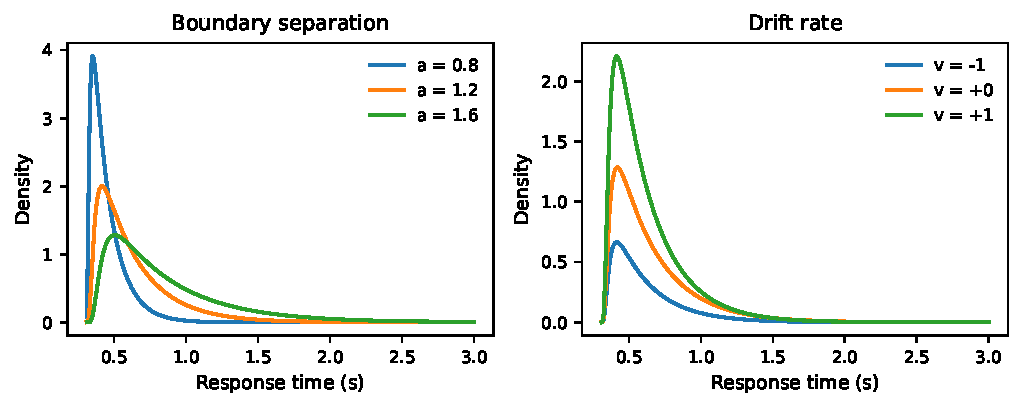
\includegraphics[width=0.88\textwidth]{figures/model_illustration.pdf}
  \caption{WFPT densities for the upper boundary. Left: increasing boundary separation $a$ shifts the distribution to the right and thickens the tail. Right: increasing drift $v$ shifts the distribution to the left and increases the probability of the upper response. The non-decision time is fixed at $t_0=0.3$\,s.}
  \label{fig:model}
\end{figure}

\subsection{Estimation and the limits of existing tools}

Given trial-level data $\{(RT_i,c_i)\}_{i=1}^N$, MLE maximizes
\begin{equation}
  \ell(v,a,w,t_0)
  =
  \sum_{i=1}^{N}
  \log f_{c_i}(RT_i\mid v,a,w,t_0),
  \label{eq:loglik}
\end{equation}
where $f_{c_i}$ is the density of the chosen boundary. For multiple subjects, one can fit a separate parameter vector per subject; the likelihood is separable, but a batched implementation can evaluate all subjects in one graph.

The main alternatives embody different trade-offs. \texttt{fast-dm} is a mature C implementation with ML, chi-square, and Kolmogorov--Smirnov criteria \citep{Voss2015}. \texttt{HDDM} is hierarchical Bayesian and therefore provides shrinkage and posterior uncertainty, at the cost of MCMC \citep{Wiecki2013}. \texttt{PyDDM} uses numerical PDE solutions to support generalized drift, noise, and boundary functions \citep{Shinn2020}. \texttt{fddm} provides highly optimized C++ density and derivative routines \citep{FosterSingmann2024}. GPU acceleration has been demonstrated for a different diffusion model with bounded gradient drift \citep{Loossens2022}, but standard DDM tooling for Apple GPUs is sparse. Moment-based methods such as EZ-diffusion are much faster than full likelihood fitting, but they rely on summary statistics and restrictive assumptions \citep{Wagenmakers2007}.

A differentiable likelihood is useful beyond MLE. It enables gradient-based variational inference \citep{Blei2017,Kucukelbir2017}, trial-level regression through the parameters, neural-network amalgamation, and amortized inference \citep{Wu2026}. Recent work has also examined the robustness of amortized estimators to contaminant observations \citep{WuRadev2024}. Our implementation is a step toward that ecosystem, not a replacement for the mature tools above.

\section{Implementation}

\subsection{Vectorized WFPT density}

The public function \texttt{wfpt\_logpdf} accepts response times and parameters as Python scalars or broadcastable tensors. Internally, all inputs are broadcast to a common shape, the effective decision time $\tau=RT-t_0$ is formed, and the hybrid expansion is evaluated in log space:
\begin{align}
  \log f_\ell(t)
  &=
  \log\pi - 2\log a - vaw - \frac{v^2t}{2}
  + \log\!\left(\sum_{k=1}^{K} k\sin(k\pi w)e^{-k^2\pi^2t/(2a^2)}\right),
  \label{eq:loglarge}\\
  \log f_s(t)
  &=
  \log a - \frac{1}{2}\log(2\pi) - \frac{3}{2}\log t - vaw - \frac{v^2t}{2}
  + \log\!\left(\sum_{j=-K}^{K}(w+2j)e^{-a^2(w+2j)^2/(2t)}\right).
  \label{eq:logsmall}
\end{align}
The sums are computed as tensor contractions over the series index, so the cost is linear in the number of trials and independent of the number of subjects at the level of the graph. Parameters are clamped to their mathematical domains only at the boundary; interior optima are unaffected. Trials with $RT\le t_0$ receive a large negative log density rather than a NaN.

Two numerical details matter. First, the large-time and small-time sums are evaluated in float32 on MPS and float64 on CPU; PyTorch's MPS backend does not support float64. Second, the small-time series can underflow for extremely small $\tau/a^2$, where the true density is below the representable range of float32. The series sum is therefore clamped at \texttt{torch.finfo(dtype).tiny} (approximately $1.18\times10^{-38}$ for float32) before its logarithm is taken. This prevents \texttt{-inf} and bounds $\log(\text{sum})$ from below by $\log(\text{tiny})\approx-87.3$; the additive log multiplier can shift the resulting log density further. This is a numerical guard, not a model for the extreme tail. In the 20,000-case validation, only two reference densities fell below the float32 range. Section~\ref{sec:density-validation} quantifies the error for representable cases.

\subsection{Likelihood and choice coding}

For a trial with choice $c_i\in\{0,1\}$, we use
\begin{equation}
  v_i =
  \begin{cases}
    -v, & c_i=1,\\
    v, & c_i=0,
  \end{cases}
  \qquad
  w_i =
  \begin{cases}
    1-w, & c_i=1,\\
    w, & c_i=0.
  \end{cases}
  \label{eq:choice-transform}
\end{equation}
Then $\log f_{c_i}(RT_i)=\log f_{\mathrm{lower}}(RT_i\mid v_i,a,w_i,t_0)$, which avoids branching over trials and keeps the computation fully vectorized. The analytic choice probability in Equation~\eqref{eq:pupper} is exposed separately and is used by the sampler and by tests.

The likelihood can optionally include a fixed-proportion uniform contaminant.  For a contaminant probability $p\in[0,1)$, the mixture density is
\begin{equation}
  f_{\mathrm{mix}}(RT_i,c_i)
  =
  (1-p)f_{\mathrm{DDM}}(RT_i,c_i)
  +
  p\,\frac{1}{2(c_{\max}-c_{\min})}
  \mathbf 1[c_{\min}\le RT_i\le c_{\max}],
  \label{eq:mixture}
\end{equation}
which is evaluated with \texttt{logaddexp}.  This is a simple lapse model, not a full contaminant distribution; the contaminant probability is fixed rather than estimated.  It is used in the empirical application to match the PyDDM tutorial's 2\% uniform mixture.

\subsection{Parameterization and optimization}

We optimize unconstrained parameters $(\tilde v,\tilde a,\tilde w,\tilde t_0)$ and map them back:
\begin{equation}
  v=\tilde v,\qquad
  a=\operatorname{softplus}(\tilde a)+a_{\min},\qquad
  w=\sigma(\tilde w),\qquad
  t_0=t_{0,\max}\,\sigma(\tilde t_0),
  \label{eq:transforms}
\end{equation}
where $\sigma$ is the logistic function, $a_{\min}=0.05$ keeps the boundary separation strictly positive and well below plausible fitted values, and $t_{0,\max}=0.999\min_i RT_i$ by default.  When a contaminant mixture is used, $t_{0,\max}$ can be set independently; we fixed it at 0.6\,s in both empirical analyses to use a common bound across the two datasets.  This value was chosen before fitting and is not estimated; a sensitivity analysis over $t_{0,\max}$ is not reported.  The last constraint guarantees $RT_i>t_0$ for every trial while allowing $t_0$ to approach the fastest response. It is a numerical device, not a theoretical claim about the non-decision time distribution.

The transformations are smooth bijections, so they keep the parameters in their domains without hard constraints during optimization. Near the upper bound the logistic derivative approaches zero, which can slow optimization when $t_0$ is close to $t_{0,\max}$; this is a known trade-off of the reparameterization. The hard clamps in the density are only a fallback for numerical overflow and are inactive at interior optima.

The default optimizer is LBFGS with strong Wolfe line search \citep{NocedalWright2006}, which is well suited to a smooth, deterministic full-batch objective. If LBFGS raises a runtime error---for example, because a line search encounters a non-finite value---the implementation falls back to Adam. Multiple random restarts are supported but off by default. For $S$ subjects, the parameter tensor has shape $S\times 4$ and trial-level parameters are gathered by subject index, so all subjects are optimized jointly. This is a \emph{pooled independent-subject} MLE, not a hierarchical model: there is no shrinkage and no group-level distribution.

\subsection{Simulation and software}

Synthetic data can be generated in two ways. The fast path inverts the WFPT CDF on a dense grid, vectorized over trials; the slower path integrates the SDE with Euler--Maruyama. The grid sampler is convenient for large recovery studies, but because it uses the same density as the likelihood, it constitutes an ``inverse crime'' if used alone. We therefore also report a recovery study based on Euler--Maruyama data, which is numerically independent of the likelihood, albeit discretized.

The package is pure Python with no compiled dependencies beyond PyTorch. Listing~\ref{lst:api} shows the core API. The repository includes tests for density correctness, gradients, sampler moments, parameter recovery, and CPU/MPS agreement.

\begin{lstlisting}[caption={Minimal \texttt{ddmtorch} workflow.},label={lst:api}]
import torch
from ddmtorch import fit_mle, sample_wfpt

rt, choice = sample_wfpt(v=1.0, a=1.2, w=0.5, t0=0.3,
                         n=2000, device="cpu")
fit = fit_mle(rt, choice, device="mps")
print(fit.params)   # columns: v, a, w, t0
\end{lstlisting}

\section{Experiments}

\subsection{Density validation}
\label{sec:density-validation}

We generated 20,000 random parameter sets with $t_0\in[0.1,0.5]$, $\tau\in[0.005,3.0]$, $v\in[-2,2]$, $a\in[0.6,2.0]$, and $w\in[0.15,0.85]$. The reference was a CPU float64 evaluation with $k_{\max}=512$; the production implementation used $k_{\max}=48$ on CPU float32 and MPS float32. For the 19,918 cases with $\tau\ge0.02$ and a reference density representable in float32, the maximum absolute log-density error was $3.51\times10^{-5}$ on CPU float32 and $3.13\times10^{-5}$ on MPS; the corresponding mean absolute errors were $5.2\times10^{-7}$ and $6.3\times10^{-7}$. CPU float32 and MPS float32 agreed to $7.6\times10^{-6}$ in log density. Two of the 82 cases with $\tau<0.02$ also had reference densities below the float32 range; among the remaining representable cases in that group, the maximum error was $1.1\times10^{-4}$.

We also checked the small-time truncation separately: in the 9,835 cases where the small-time expansion is used, increasing the sum from $j=-48,\ldots,48$ to $j=-256,\ldots,256$ produced no change at float64 precision (maximum absolute log-density error 0). This is expected because terms beyond $|j|=48$ underflow in the tested range. The truncation is therefore not a source of error here, although it should be rechecked if the parameter range is extended.

This is sufficient for likelihood-based estimation in the tested range, but it is not a claim of float64-level accuracy. For publication-grade numerical work, or for data with responses extremely close to $t_0$, the CPU float64 backend should be used.

\subsection{Synthetic parameter recovery}

We generated 100 datasets with 500 trials each. True parameters were drawn uniformly from $v\in[-2,2]$, $a\in[0.7,2.0]$, $w\in[0.35,0.65]$, and $t_0\in[0.10,0.50]$. Data were generated with the grid sampler ($n_{\mathrm{grid}}=8192$) and fitted on MPS with LBFGS. All 100 fits returned finite solutions. Table~\ref{tab:recovery} and Figure~\ref{fig:recovery} summarize recovery. The correlations were $r=0.996$ for $v$, $0.995$ for $a$, $0.981$ for $w$, and $0.998$ for $t_0$; RMSEs were $0.097$, $0.034$, $0.018$, and $0.007$, respectively. Mean fit time was 0.34\,s per dataset.

\begin{table}[H]
\centering
\caption{Synthetic parameter recovery. Main study: 100 datasets $\times$ 500 trials, grid sampler, MPS fit. Independent check: 100 datasets $\times$ 500 trials, Euler--Maruyama sampler ($dt=10^{-3}$), MPS fit.}
\label{tab:recovery}
\begin{tabular}{lcccccc}
\toprule
 & \multicolumn{2}{c}{Main study} & & \multicolumn{2}{c}{Euler check} & \\
\cmidrule(lr){2-3}\cmidrule(lr){5-6}
Parameter & RMSE & $r$ & & RMSE & $r$ & \\
\midrule
Drift rate $v$ & 0.097 & 0.996 & & 0.101 & 0.997 & \\
Boundary $a$ & 0.034 & 0.995 & & 0.049 & 0.995 & \\
Start point $w$ & 0.018 & 0.981 & & 0.018 & 0.980 & \\
Non-decision $t_0$ & 0.007 & 0.998 & & 0.007 & 0.998 & \\
\bottomrule
\end{tabular}
\end{table}

\begin{figure}[H]
  \centering
  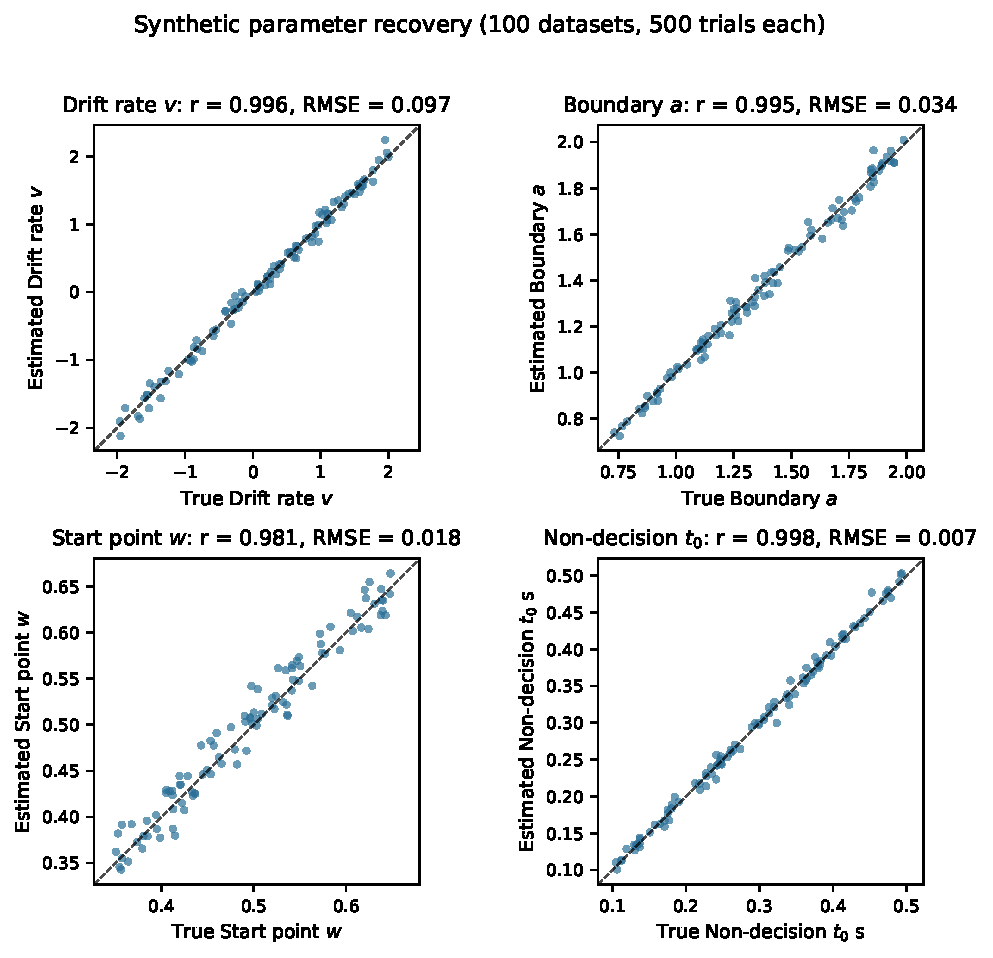
\includegraphics[width=0.82\textwidth]{figures/recovery_scatter.pdf}
  \caption{True versus estimated parameters for 100 synthetic datasets (500 trials each). Dashed lines are identity lines.}
  \label{fig:recovery}
\end{figure}

The Euler--Maruyama check used 100 datasets, $dt=10^{-3}$, and discarded unresolved trials (0.012\% in practice). Recovery remained strong, but we observed a small positive bias in $a$ ($+0.033$) and essentially no bias in $v$ ($+0.0004$), $w$ ($+0.001$), and $t_0$ ($+0.002$). The boundary bias is consistent with boundary-crossing discretization. This check reduces, but does not eliminate, the concern that the main study is an inverse crime: the likelihood is still the same parametric model, and the Euler simulator is an approximation to that model.

\subsection{Empirical application: motion discrimination}
\label{sec:empirical}

To check the implementation on real data, we used the public, processed \citet{Roitman2002} motion-discrimination dataset, which contains two monkeys, six motion-coherence levels (0 to 0.512), and 6,149 trials.  Following the PyDDM tutorial for this dataset, we removed responses faster than 100\,ms and slower than 1,650\,ms, leaving 2,611 trials for monkey 1 and 3,533 for monkey 2.  The model was a standard four-parameter DDM with drift proportional to coherence, $v_i=\beta\,\mathrm{coh}_i$, a constant boundary $a$, a free starting point $w$, and non-decision time $t_0$.  We added the fixed 2\% uniform contaminant of Equation~\eqref{eq:mixture} ($c_{\min}=0$, $c_{\max}=2$\,s) because the data contain fast responses that a no-mixture DDM in our implementation would be forced to absorb by placing $t_0$ below the fastest RT (about 0.1\,s).
In a separate synthetic check (2,000 trials, 5\% uniform contaminants, true $t_0=0.32$\,s; see the repository for the script), the no-mixture fit was forced to $t_0=0.075$\,s and $a=1.72$, whereas the 5\% mixture recovered $t_0=0.314$\,s and $a=1.20$ (true $a=1.20$).  This check is illustrative rather than a full recovery study, but it shows why the mixture matters.

PyDDM parameterizes a symmetric bound as \([-B,B]\) and normalizes its starting-point parameter \(x_0\) to \([-1,1]\), with \(x_0=0\) unbiased.  We therefore convert \(a=2B\) and \(w=x_0/2+0.5\); no assumption that \(B=1\) is involved.

We fitted each monkey separately with \texttt{ddmtorch} (MPS, LBFGS, three restarts) and with PyDDM 0.9.0 (CPU, Fokker--Planck solver, same model and mixture).  Table~\ref{tab:empirical} and Figure~\ref{fig:empirical} show the results.  The two implementations recovered nearly identical parameters.  For monkey 1, \texttt{ddmtorch} gave $\beta=10.49$, $a=1.49$, $w=0.488$, and $t_0=0.307$; PyDDM gave $\beta=10.54$, $a=1.49$, $w=0.483$, and $t_0=0.309$.  For monkey 2, the estimates were $\beta=9.49$, $a=1.75$, $w=0.501$, $t_0=0.193$ and $\beta=9.60$, $a=1.75$, $w=0.494$, $t_0=0.194$, respectively.  The total negative log likelihoods were also close: 204.30 versus 206.66 for monkey 1, and 1254.22 versus 1254.61 for monkey 2.  Both values are total negative log-likelihoods over trials under the same mixture model; PyDDM's default likelihood loss sums trial-level log densities.  The small differences may therefore reflect the different numerical routes (closed-form WFPT series versus a Fokker--Planck PDE), discretization settings, and mixture implementations; they are not evidence that one implementation is more correct.

Because \texttt{ddmtorch} used three restarts while PyDDM used its default optimizer, the wall-clock times in Table~\ref{tab:empirical} are descriptive only and should not be read as a like-for-like speed comparison.

\begin{table}[H]
\centering
\caption{Empirical application to the Roitman and Shadlen (2002) dataset.  The model is $v_i=\beta\,\mathrm{coh}_i$ with a constant boundary, free starting point, non-decision time, and a fixed 2\% uniform contaminant.  Units: $\beta$ in evidence/s, $a$ in evidence units, $w$ dimensionless, and $t_0$ in seconds.  For PyDDM, $a=2B$ converts its symmetric bound to boundary separation, and $w=x_0/2+0.5$, where PyDDM's \(x_0\) is normalized to \([-1,1]\).  Times are wall-clock for the full fitting procedure; \texttt{ddmtorch} used three restarts, PyDDM used its default optimizer, so timings are not directly comparable.}
\label{tab:empirical}
\begin{tabular}{llrrrrrr}
\toprule
Monkey & Method & $\beta$ & $a$ & $w$ & $t_0$ & Total NLL & Time (s) \\
\midrule
1 & \texttt{ddmtorch} & 10.494 & 1.489 & 0.488 & 0.307 & 204.30 & 2.65 \\
1 & PyDDM & 10.536 & 1.486 & 0.483 & 0.309 & 206.66 & 3.92 \\
2 & \texttt{ddmtorch} & 9.495 & 1.749 & 0.501 & 0.193 & 1254.22 & 1.50 \\
2 & PyDDM & 9.602 & 1.754 & 0.494 & 0.194 & 1254.61 & 2.88 \\
\bottomrule
\end{tabular}
\end{table}

\begin{figure}[H]
  \centering
  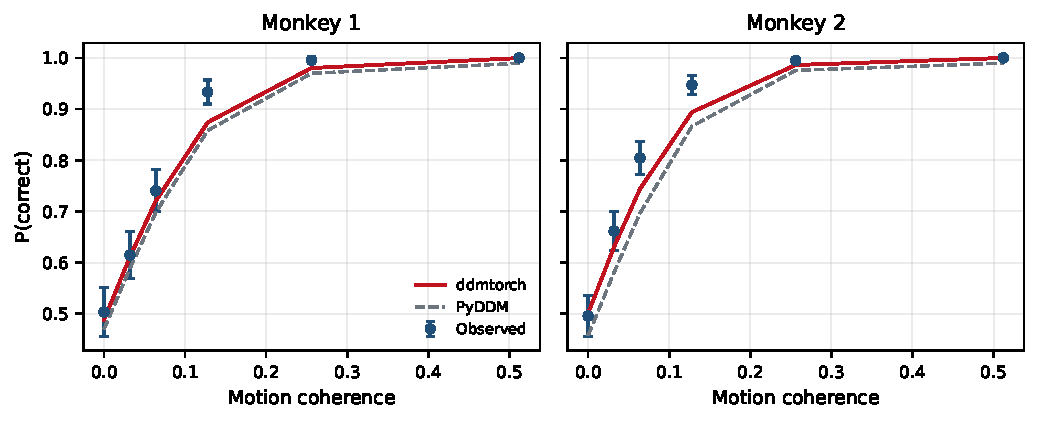
\includegraphics[width=0.88\textwidth]{figures/empirical_psychometric.pdf}
  \caption{Observed and predicted psychometric functions for the Roitman and Shadlen (2002) data.  Error bars are 95\% binomial intervals.  Both implementations produce nearly identical predictions.  The simple constant-bound DDM under-predicts accuracy at intermediate coherences, especially for monkey 2; this is a property of the model, not of either implementation, and motivates across-trial variability or collapsing bounds.}
  \label{fig:empirical}
\end{figure}

Table~\ref{tab:bootstrap} reports 95\% percentile intervals from 500 trial-level bootstrap resamples per monkey.  Each resample was refitted with \texttt{ddmtorch}, initialized at the full-data estimate; PyDDM intervals were not bootstrapped.  The intervals are narrow because each monkey contributes thousands of trials, and they describe trial-level sampling variability, not between-subject variability.  They condition on the fixed 2\% contaminant probability and on the DDM being the true model; they do not represent model uncertainty.  Trial-level resampling also assumes that trials are exchangeable within a monkey; if trials are correlated within sessions, these intervals may understate uncertainty.  The processed file does not include session labels, so a session-level bootstrap was not possible.

\begin{table}[H]
\centering
\caption{Bootstrap percentile intervals for the \texttt{ddmtorch} empirical fits (500 resamples per monkey).  Intervals are trial-level nonparametric bootstrap percentile intervals.  $\beta$ is in evidence/s, $a$ in evidence units, and $t_0$ in seconds; $w$ is dimensionless.}
\label{tab:bootstrap}
\begin{tabular}{llrr}
\toprule
Monkey & Parameter & Estimate & 95\% bootstrap CI \\
\midrule
1 & $\beta$ & 10.494 & [10.050, 11.048] \\
1 & $a$ & 1.489 & [1.458, 1.511] \\
1 & $w$ & 0.488 & [0.479, 0.498] \\
1 & $t_0$ & 0.307 & [0.301, 0.319] \\
2 & $\beta$ & 9.495 & [9.158, 9.939] \\
2 & $a$ & 1.749 & [1.726, 1.770] \\
2 & $w$ & 0.501 & [0.491, 0.511] \\
2 & $t_0$ & 0.193 & [0.189, 0.198] \\
\bottomrule
\end{tabular}
\end{table}

Figure~\ref{fig:rt-quantiles} compares observed and predicted RT quantiles (0.1, 0.3, 0.5, 0.7, 0.9) for correct and error responses at each coherence level.  The model over-disperses RTs at low coherence and over-predicts the slow tail at high coherence; the RMSE across the 100 quantile points was 0.165\,s.  Because the two implementations produce nearly identical parameter estimates, their predicted quantiles are expected to agree closely; the misfit is therefore more likely a model limitation than an implementation disagreement.

\begin{figure}[H]
  \centering
  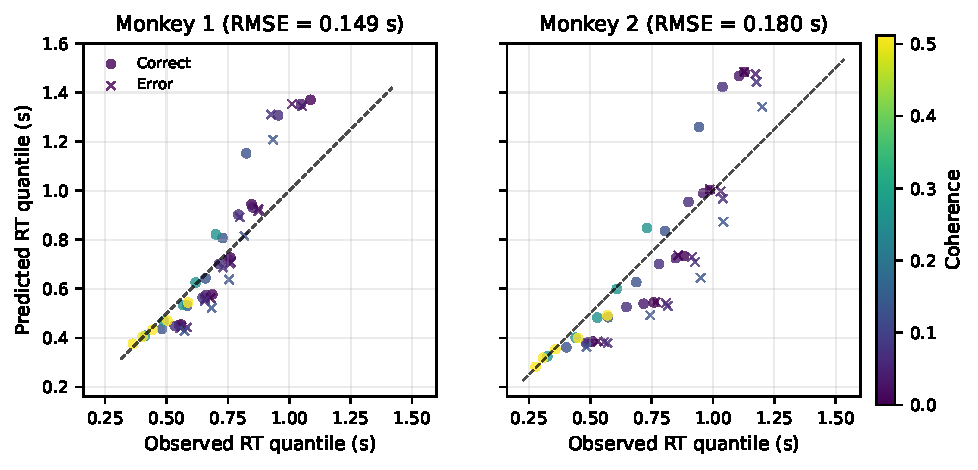
\includegraphics[width=0.88\textwidth]{figures/empirical_rt_quantiles.pdf}
  \caption{Observed versus predicted RT quantiles for the Roitman and Shadlen (2002) data.  Each point is one quantile (0.1, 0.3, 0.5, 0.7, 0.9) for correct (circles) or error (crosses) responses at a given coherence level; color encodes coherence.  Predictions come from the \texttt{ddmtorch} fit.  Points on the dashed line indicate perfect agreement.  The systematic deviations are more likely a property of the simple constant-bound model than an implementation difference.}
  \label{fig:rt-quantiles}
\end{figure}

The empirical application also exposes a substantive limitation.  Both toolboxes agree, but both under-predict the steep rise in accuracy at intermediate coherences for monkey 2 (Figure~\ref{fig:empirical}).  Adding across-trial variability, a collapsing bound, or a more flexible drift function would be needed to capture that pattern.  This is exactly the kind of model-development loop that a fast, differentiable likelihood is meant to support.

\subsection{Hierarchical comparison on a multi-subject dataset}
\label{sec:hierarchical}

The Roitman application is a single task with two monkeys, so it cannot assess hierarchical inference.  We therefore used the \citet{Cavanagh2011} reward-based decision dataset distributed with the HDDM examples.  It contains 14 subjects, three stimulus conditions (LL, WL, WW), and 3,988 trials; responses are coded as 0/1 and RTs range from 0.40 to 4.84\,s.  We fit an HDDM-style hierarchical DDM with subject-specific drift rates for the three conditions, subject-specific boundary and non-decision time, a fixed starting point $w=0.5$, and a fixed 5\% uniform contaminant (HDDM's default outlier probability).

Let $s=1,\ldots,14$ index subjects and $c\in\{\mathrm{LL},\mathrm{WL},\mathrm{WW}\}\).  The non-centered priors were
\begin{align}
  v_{s,c} &= \mu_{v,c} + \sigma_{v,c}\tilde v_{s,c}, & \tilde v_{s,c} &\sim N(0,1), \label{eq:hier-v}\\
  a_s &= \exp(\mu_{\log a} + \sigma_{\log a}\tilde a_s), & \tilde a_s &\sim N(0,1), \label{eq:hier-a}\\
  t_{0,s} &= 0.6\,\operatorname{logistic}(\mu_{t_0}+\sigma_{t_0}\tilde t_{0,s}), & \tilde t_{0,s} &\sim N(0,1), \label{eq:hier-t0}
\end{align}
with $\mu_{v,c}\sim N(0,2)$, $\sigma_{v,c}\sim\mathrm{HalfNormal}(1)$, $\mu_{\log a}\sim N(\log 1.2,0.5)$, $\sigma_{\log a}\sim\mathrm{HalfNormal}(0.5)$, $\mu_{t_0}\sim N(0,1)$, and $\sigma_{t_0}\sim\mathrm{HalfNormal}(0.5)$.  The model was fitted with PyMC 5 \citep{AbrilPla2023} and the nutpie NUTS backend.\footnote{\url{https://github.com/pymc-devs/nutpie}}  As of October 2026, HDDM 1.0.1 (released December 2023) depends on PyMC 2, and we could not install it on Apple Silicon/macOS; we did not attempt a Linux or containerized installation.  This is therefore an HDDM-style reimplementation of the model class, not a run of the HDDM package.

We drew 1,000 samples after 1,000 tuning samples in four chains.  The maximum R-hat was 1.005 and the minimum bulk effective sample size was 500; this is reasonably converged for the present comparison, though it remains a reimplementation rather than a definitive HDDM posterior.  We also fitted each subject separately with \texttt{ddmtorch} using the same model, five parameters per subject (three drift rates, boundary, non-decision time), two restarts, and the same 5\% contaminant; both fits bound the non-decision time at 0.6\,s.  Three of the 14 MLEs (subjects 7, 10, and 11) reached that bound, so the $t_0$ comparison should be read with this constraint in mind.  Mean MLE time was 0.48\,s per subject.

Table~\ref{tab:hierarchical} and Figure~\ref{fig:hierarchical} show the agreement.  Across subjects, the correlations were $r=0.997$ ($v_{\mathrm{LL}}$), $0.9995$ ($v_{\mathrm{WL}}$), $0.997$ ($v_{\mathrm{WW}}$), $0.999$ ($a$), and $0.996$ ($t_0$); RMSEs were 0.065, 0.032, 0.074, 0.015, and 0.009, respectively.  The hierarchical estimates were less dispersed than the MLEs for $v_{\mathrm{LL}}$ (SD 0.161 vs 0.226), $v_{\mathrm{WW}}$ (0.233 vs 0.307), and $t_0$ (0.094 vs 0.097), consistent with shrinkage; $v_{\mathrm{WL}}$ showed modest shrinkage, and $a$ showed little.  This is the expected qualitative behavior when individual estimates are pulled toward a group distribution.

\begin{table}[H]
\centering
\caption{Agreement between \texttt{ddmtorch} per-subject MLE and the PyMC 5 HDDM-style hierarchical fit on the 14-subject \citet{Cavanagh2011} dataset.  Correlations and RMSE are computed across the 14 subjects; for $v$, each row is a separate stimulus condition.  SD columns show the between-subject spread of the estimates.  Drift rates are in evidence/s, $a$ in evidence units, and $t_0$ in seconds.}
\label{tab:hierarchical}
\begin{tabular}{lrrrr}
\toprule
Parameter & $r$ & RMSE & MLE SD & Hier. SD \\
\midrule
$v$ (LL) & 0.997 & 0.065 & 0.226 & 0.161 \\
$v$ (WL) & 0.9995 & 0.032 & 0.351 & 0.320 \\
$v$ (WW) & 0.997 & 0.074 & 0.307 & 0.233 \\
$a$ & 0.999 & 0.015 & 0.323 & 0.318 \\
$t_0$ & 0.996 & 0.009 & 0.097 & 0.094 \\
\bottomrule
\end{tabular}
\end{table}

\begin{figure}[H]
  \centering
  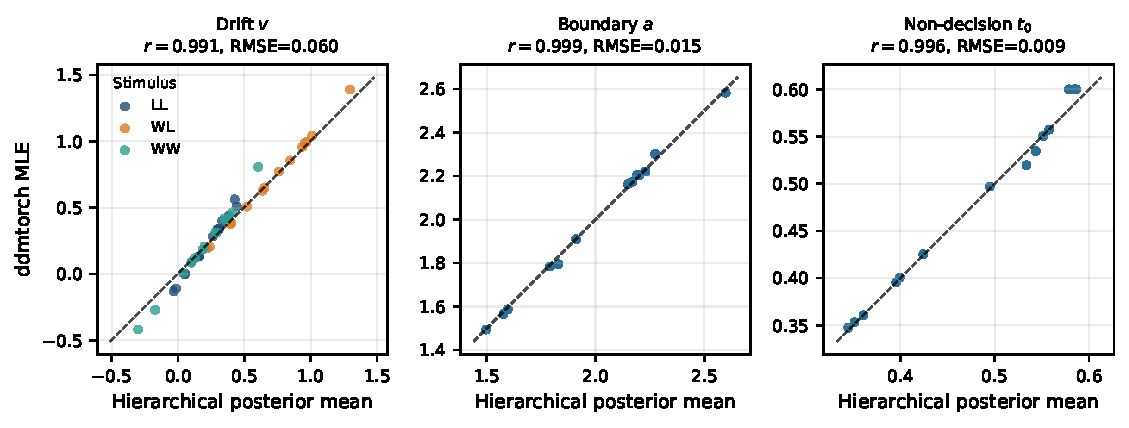
\includegraphics[width=0.92\textwidth]{figures/hierarchical_comparison.pdf}
  \caption{\texttt{ddmtorch} per-subject MLE versus PyMC 5 hierarchical posterior means for the 14-subject \citet{Cavanagh2011} dataset.  Left: drift rates by stimulus condition.  Middle: boundary.  Right: non-decision time.  Dashed lines are identity lines.  The drift panel pools the three conditions ($r=0.991$); the correlations in Table~\ref{tab:hierarchical} range from $0.996$ to $0.9995$.  The lower pooled correlation reflects the different drift ranges across conditions, not poorer estimation within conditions.  The hierarchical estimates are slightly less dispersed, consistent with shrinkage.}
  \label{fig:hierarchical}
\end{figure}

The pooled drift correlation in Figure~\ref{fig:hierarchical} is lower than the condition-specific correlations because the LL, WL, and WW conditions have different mean drift rates; pooling them adds between-condition variance and is not a measure of within-condition estimation quality.  The comparison has clear limits.  It is a reimplementation, not a direct HDDM benchmark; the hierarchical model fixes $w=0.5$; and a longer MCMC run could refine the posterior.  It nevertheless shows that \texttt{ddmtorch}'s point estimates agree with a hierarchical Bayesian fit of the same model class, and that the differences are in the direction expected from shrinkage.  A direct comparison with the HDDM software, and a longer hierarchical run, remain future work.

\subsection{CPU and MPS benchmarks}
\label{sec:benchmarks}

Benchmarks were run on a MacBook Air with an Apple M5 chip, 24\,GB unified memory, macOS 26.5, Python 3.12.16, and PyTorch 2.14.1. We measured forward and backward passes through the WFPT log likelihood, and full MLE fits. Timings include the optimizer for MLE and were synchronized with \texttt{torch.mps.synchronize()} for MPS. Each density timing is the mean of five iterations after warm-up.

\begin{table}[H]
\centering
\caption{Selected benchmarks. Density: forward + backward time for the WFPT likelihood. MLE: wall-clock time for a full fit. The 50k MLE used 20 subjects with 2,500 trials each. Density timings were collected at 1k, 10k, 100k, and 1M trials (the 1k row is omitted for space); MLE timings at 2k, 10k, and 50k trials. Dashes indicate combinations that were not run.}
\label{tab:bench}
\begin{tabular}{lrrrrrr}
\toprule
 & \multicolumn{3}{c}{Density (s)} & \multicolumn{3}{c}{MLE (s)} \\
\cmidrule(lr){2-4}\cmidrule(lr){5-7}
Trials & CPU64 & CPU32 & MPS & CPU64 & CPU32 & MPS \\
\midrule
2,000 & -- & -- & -- & 1.04 & 0.12 & 0.26 \\
10,000 & 0.021 & 0.020 & 0.003 & 0.66 & 0.46 & 0.28 \\
100,000 & 0.232 & 0.109 & 0.067 & -- & -- & -- \\
1,000,000 & 3.21 & 1.22 & 0.62 & -- & -- & -- \\
50,000 (20 subj.) & -- & -- & -- & 7.30 & 4.10 & 2.32 \\
\bottomrule
\end{tabular}
\end{table}

\begin{figure}[H]
  \centering
  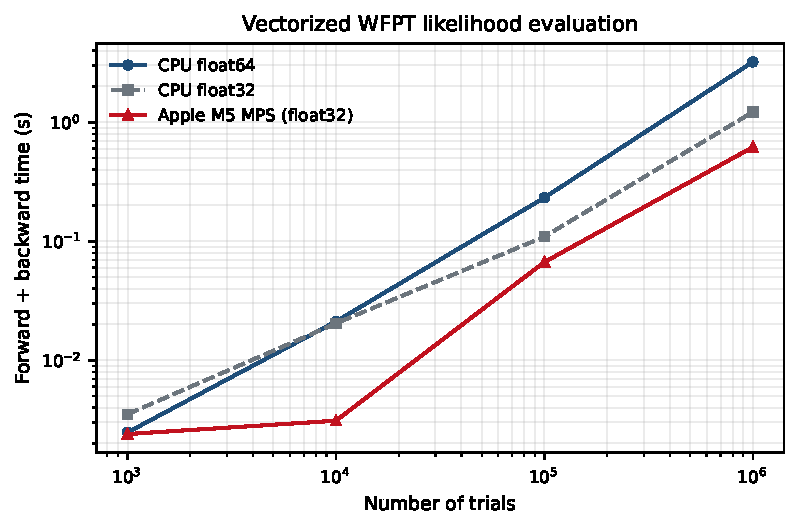
\includegraphics[width=0.72\textwidth]{figures/benchmark_scaling.pdf}
  \caption{Forward + backward time for the vectorized WFPT likelihood as a function of the number of trials. Both axes are logarithmic.}
  \label{fig:scaling}
\end{figure}

\begin{figure}[H]
  \centering
  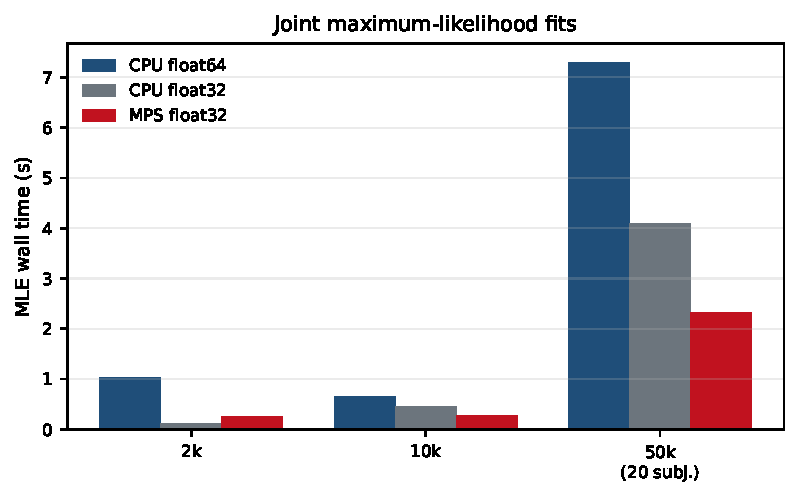
\includegraphics[width=0.72\textwidth]{figures/benchmark_mle.pdf}
  \caption{Wall-clock time for full MLE fits. The 50k condition uses 20 subjects.}
  \label{fig:mle}
\end{figure}

The pattern is clear. At one million trials, MPS is 1.97$\times$ faster than CPU float32 and 5.20$\times$ faster than CPU float64 for a forward--backward pass. At 50,000 trials with 20 subjects, MPS is 1.77$\times$ faster than CPU float32 and 3.15$\times$ faster than CPU float64 for a full MLE fit. For small workloads, however, CPU float32 wins: a 2,000-trial MLE takes 0.12\,s on CPU versus 0.26\,s on MPS, because kernel-launch and synchronization overhead dominate. At 10,000 trials, MPS is about 1.6$\times$ faster than CPU float32, while at 2,000 trials CPU float32 is about 2.2$\times$ faster. This is not a defect of the implementation; it is the expected shape of the CPU/GPU trade-off. Users should choose the backend based on trial count, precision requirements, and whether they need float64.

\subsection{What the benchmark does and does not show}

The benchmark is an internal CPU-versus-MPS comparison on one machine. It is not a head-to-head speed comparison with \texttt{fddm}, \texttt{fast-dm}, \texttt{HDDM}, or \texttt{PyDDM}; the empirical section compares parameter estimates with \texttt{PyDDM}, but not wall-clock speed.  Those tools use different algorithms, fitting criteria, and hardware assumptions, and a fair speed comparison would require a separate study. It also does not benchmark CUDA, because no NVIDIA GPU was available. The CPU float32 condition is included precisely to avoid the misleading impression that MPS is five times faster than all CPU code; against the same precision, the speedup is roughly twofold at large batch sizes.

\section{Discussion}

\subsection{What the toolbox enables}

\texttt{ddmtorch} makes three practical workflows easier on a Mac. First, a researcher can fit a standard DDM to a multi-subject dataset with a few lines of code and no compiled dependencies beyond PyTorch. Second, because the likelihood is differentiable, the same code can be embedded in a larger PyTorch model---for example, a neural network that predicts trial-wise drift rates, or a variational inference procedure over subject parameters. Third, the vectorized design makes large simulation studies and parameter-recovery checks inexpensive, which is useful for teaching and for pre-registering analysis plans.

The recovery results suggest that the implementation is accurate enough for standard applications in the tested parameter range. The density validation shows that MPS float32 is not merely a fast approximation: it agrees with a float64 reference to within $3\times10^{-5}$ in log density over the bulk of the parameter space. The speedups are largest exactly where they matter most---large trial counts and multi-subject fits.

\subsection{Limitations}

\textbf{Model scope.} We implement the standard four-parameter DDM with fixed boundaries, constant drift, and no across-trial variability. The full Ratcliff model includes inter-trial variability in drift ($s_v$), starting point ($s_z$), and non-decision time ($s_t$), as well as contaminant responses \citep{RatcliffMcKoon2008}. These extensions are not optional details: they change the shape of the RT distribution and can materially affect parameter estimates. \texttt{HDDM}, \texttt{fast-dm}, and \texttt{PyDDM} support various subsets of the variability parameters; \texttt{ddmtorch} does not.  The package does support a fixed-proportion uniform contaminant (used in Section~\ref{sec:empirical}), but the contaminant probability is not estimated and the contaminant distribution is deliberately simple.  Nor do we implement collapsing bounds, time-varying drift, or reinforcement-learning extensions \citep{Fengler2022}.

\textbf{Inference scope.} We provide point estimates from MLE, not posterior distributions.  The core API does not compute standard errors; for the empirical application we report bootstrap percentile intervals.  There is no hierarchical shrinkage or posterior uncertainty, and no model-comparison machinery. For many research questions---especially with few trials per subject---a hierarchical Bayesian model is preferable \citep{Wiecki2013,Vandekerckhove2011}. Variational inference is a promising middle ground \citep{Blei2017,Kucukelbir2017}, and amortized inference can make repeated inference nearly instantaneous \citep{Wu2026}, but neither is implemented here.

\textbf{Numerical scope.} MPS runs in float32. The density is accurate in the tested range, but extreme right-tail values can underflow, and responses very close to $t_0$ should be checked with CPU float64. The $t_0$ constraint $t_0<0.999\min_i RT_i$ is a numerical device; when no mixture is used, it can bias $t_0$ downward if the fastest response is a contaminant.  The empirical fits fix $t_{0,\max}=0.6$\,s before fitting; we did not run a sensitivity analysis over this bound, so estimates near 0.6\,s should be interpreted cautiously.  The core API supports a fixed-proportion uniform contaminant, but the contaminant probability is not estimated.

\textbf{Evidence scope.} The recovery study is synthetic.  The Roitman application contains only two monkeys from one task, and the hierarchical comparison uses 14 subjects from a different task and a PyMC 5 reimplementation rather than the HDDM package.  We compared against PyDDM and the hierarchical reimplementation, but not against \texttt{HDDM} or \texttt{fast-dm}.  The hierarchical MCMC run used four chains with 1,000 draws (maximum R-hat 1.005, minimum bulk ESS 500); it is reasonably converged for the present comparison but remains a reimplementation, not a definitive HDDM benchmark.  The Euler--Maruyama check mitigates the inverse-crime concern but introduces its own discretization bias.  The benchmark is a single-machine comparison, not a general performance claim.  Recovery is also optimistic because the generating model is correctly specified and the simulated error rates are not extreme; parameter identifiability can be poor when error rates are low, especially with few trials \citep{Lucken2025}.

\subsection{Future work}

The most valuable next step is to add across-trial variability. One route is numerical integration over the variability distributions, as in the full Ratcliff model; another is to use the derivative routines and approximations developed for \texttt{fddm} \citep{FosterSingmann2024,Blurton2017}. A second step is hierarchical Bayesian or variational inference: a mean-field Gaussian over transformed subject parameters would be straightforward with the existing differentiable likelihood, and a hierarchical prior would add shrinkage. A third step is amortized inference: train a neural posterior estimator on simulated DDM data and use the likelihood for importance correction or consensus \citep{Wu2026}. A fourth step is trial-level regression, in which $v$, $a$, or $t_0$ is a function of covariates; this is where the differentiable design pays off most clearly. Finally, a systematic comparison with \texttt{fddm}, \texttt{fast-dm}, \texttt{HDDM}, and \texttt{PyDDM} on shared datasets and the same fitting criteria would turn the present engineering report into a proper benchmark paper.

\subsection{Reproducibility and availability}

The repository contains the package, tests, experiment scripts, and the exact commands used to produce the tables and figures. The main environment is a Miniforge conda environment with Python 3.12 and PyTorch 2.14.1. The results in this report were generated on the machine described in Section~\ref{sec:benchmarks}.

All stochastic experiments use fixed seeds exposed by the scripts. The density validation used seed 123; the main recovery study used 2026, with dataset $i$ generated and fitted using 2026+$i$; the Euler check used 77, with dataset $i$ using 77+$i$; the Roitman bootstrap used 2026, with resample $b$ fitted using 2026+$b$; and the hierarchical MCMC run used 2026. The Roitman fits used restart seed 0 for \texttt{ddmtorch} and seed 0 for PyDDM's differential-evolution optimizer; the Cavanagh per-subject fits used restart seed 0. The benchmark generator used 1234 for density timings and 11 for MLE timings. The script defaults are the source of truth, and the committed \texttt{results/} files record these seeds where applicable.

\section{Conclusion}

\texttt{ddmtorch} is a focused engineering contribution toward differentiable, GPU-accelerated DDM estimation on the laptops that many cognitive scientists actually use. It does not replace \texttt{HDDM}, \texttt{fast-dm}, \texttt{PyDDM}, or \texttt{fddm}, and it does not yet implement the full Ratcliff model. What it does provide is a vectorized WFPT likelihood, a batched MLE routine, MPS support, and a reproducible evaluation showing where the speedups are real and where they are not. For a researcher who wants to fit a standard DDM on a Mac, embed the likelihood in a PyTorch model, or teach parameter recovery with fast synthetic data, that is already useful.

\section*{Data and code availability}

The code, tests, experiment scripts, and generated results accompany this manuscript.  The empirical analyses use the public Roitman and Shadlen (2002) dataset and the Cavanagh et al. (2011) dataset distributed with the HDDM examples; the analysis scripts download the processed CSVs on first run.  The code is released under the MIT license and is available at \url{https://github.com/KiraIch/ddmtorch}.  The manuscript is released under a CC BY 4.0 license.  Archived code: \url{https://doi.org/10.5281/zenodo.23721071}.

\section*{Author contributions}

ChiaAn Lin: conceptualization, software, validation, formal analysis, and writing.

\section*{Competing interests}

The author declares no competing interests.

\section*{Funding}

This work received no specific funding.

\section*{Ethics statement}

The empirical analyses used only publicly available data from previously published human and animal studies; no new human or animal subjects were used.

\section*{Acknowledgments}

This technical report was prepared as an independent side project. The author thanks the open-source community behind PyTorch, NumPy, and the DDM software ecosystem; any errors are the author's own.

{\footnotesize
\bibliographystyle{plainnat}
\bibliography{references}
}

\end{document}
